\section{Schema}
\label{schema}


\subsection{Domänenmodell}
Zur einheitlichen Darstellung und besseren Verständlichkeit der entwickelten Lösung wurde für diese Arbeit ein Domänenmodell aus dem Bereich E-Commerce definiert. Dieses Modell bildet ein beispielhaftes Szenario ab, das für die nachfolgenden Kapitel als Referenz dient. Die entwickelte Lösung ist jedoch nicht auf dieses spezielle Modell beschränkt, sondern kann auf beliebige andere Domänenmodelle übertragen werden, ohne dass Änderungen an der Kernfunktionalität nötig sind. Im diesem Abschnitt wird das erstellte Domänenmodell basierend auf der UML-Darstellung in Abbildung~\ref{fig:uml_modell} erläutert.

Info:
Das hier gezeigte Modell wird noch detaillierter beschrieben. Das Feedback von Herrn Gruntz bezüglich der UML-Darstellung wurde bisher noch nicht eingearbeitet.

\begin{figure}[H]
  \centering
  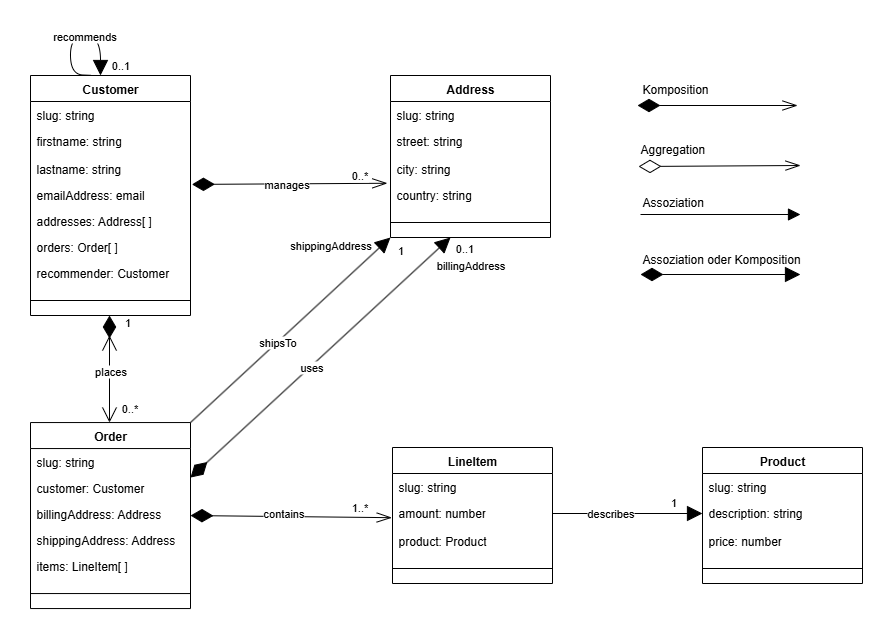
\includegraphics[width=\linewidth]{UML.png}
  \caption{UML-Darstellung des für diese Arbeit definierten Domänenmodells.}
  \label{fig:uml_modell}
\end{figure}

Das definierte Domänenmodell besteht aus den Entitäten \texttt{Customer}, \texttt{Order}, \texttt{Address}, \texttt{Product} und \texttt{LineItem}. Zur eindeutigen Identifikation im virtuellen Filesystem verfügt jede Entität zwingend über das Attribut \texttt{slug}. Der \texttt{slug} ist ein menschenlesbarer Bezeichner, der zur Generierung eindeutiger URI-Pfade verwendet wird. Wird beispielsweise ein Kunde mit dem \texttt{slug} „max“ erstellt, entsteht daraus der eindeutige URI-Pfad \texttt{/Customers/max}. Die konkrete Bedeutung und Nutzung des Attributs \texttt{slug} im Kontext des virtuellen Filesystems wird in Abschnitt~\ref{vfs-umsetzung} detailliert beschrieben.